\newpage
\section{3次元ダムブレイク}
二層流のベンチマーク問題として3次元のダムブレイク問題を解析した。

\subsection{解析条件}

Table \ref{table:dambreak-material-property}に二つの流体の物性値を示す。
Case1は水と空気の物性値である。
\renewcommand{\arraystretch}{1}
\begin{table}[H]
	\centering
	\caption{物性値}
	\begin{tabular}{ccccccc}
		\hline
		Test case & $\rho_1 (\mathrm{kg/m^3})$ & $\rho_2 (\mathrm{kg/m^3})$ & $\mu_1 (\mathrm{Ns/m^2})$& $\mu_2 (\mathrm{Ns/m^2})$ & $\mathrm{g} (\mathrm{m/s^2})$ \\
		\hline 
		Case$1$ & $998$ & $1.205$   & $1.01\times10^{-3}$ & $1.81\times10^{-5}$ & $9.81$ \\
		\hline         
	\end{tabular}
	\label{table:dambreak-material-property}
\end{table}
\renewcommand{\arraystretch}{1.0}

代表長さ$a=0.146 \mathrm{m}$として、
水柱の初期高さ$a(=0.146\mathrm{m})$、初期幅$2a(=0.292\mathrm{m})$、領域の高さ$2.4a(=0.3504\mathrm{m})$、幅$4a(=0.584\mathrm{m})$、奥行き$0.1a(=0.0146\mathrm{m})$とした。

\begin{figure}[H]
	\centering
	\includegraphics[width=10truecm]{pics/3d-dambreak/dambreak_geometry.png}
	\caption{領域の寸法\cite{Koshizuka1996}}
	\label{fig:3d-dambreak-geometry}
\end{figure}


Table \ref{table:dambreak-parameter}に解析における設定パラメータを示す。
界面幅$D$は、近似ヘビサイド関数よる平滑化の計算式(\ref{ls-heaviside})に含まれるパラメータである。
Case1と2では$D$の値が異なり、Case2の方がCase1よりも界面が平滑化される。
\renewcommand{\arraystretch}{1}
\begin{table}[H]
	\centering
	\caption{解析パラメータ}
	\begin{tabular}{cccccc}
		\hline
		Test case & $\Delta t$ & メッシュ幅$dx$ & 界面幅$D$ & 再初期化回数 & 再初期化$\Delta \tau$\\
		\hline 
		Case$1$ & $0.00025$ & $0.0146$ & $0.0438$ & $5$ & $0.0001$\\
		\hline         
	\end{tabular}
	\label{table:dambreak-parameter}
\end{table}
\renewcommand{\arraystretch}{1.0}

Figure \ref{fig:3d-dambreak-mesh}に解析用のメッシュを示す。メッシュは六面体$1$次要素を使用した。
Figure \ref{fig:3d-dambreak-boundary}に初期状態のレベルセット関数と、境界条件を示す。

\begin{figure}[H]
	\centering
	\begin{minipage}[b]{0.49\columnwidth}
	    \centering
		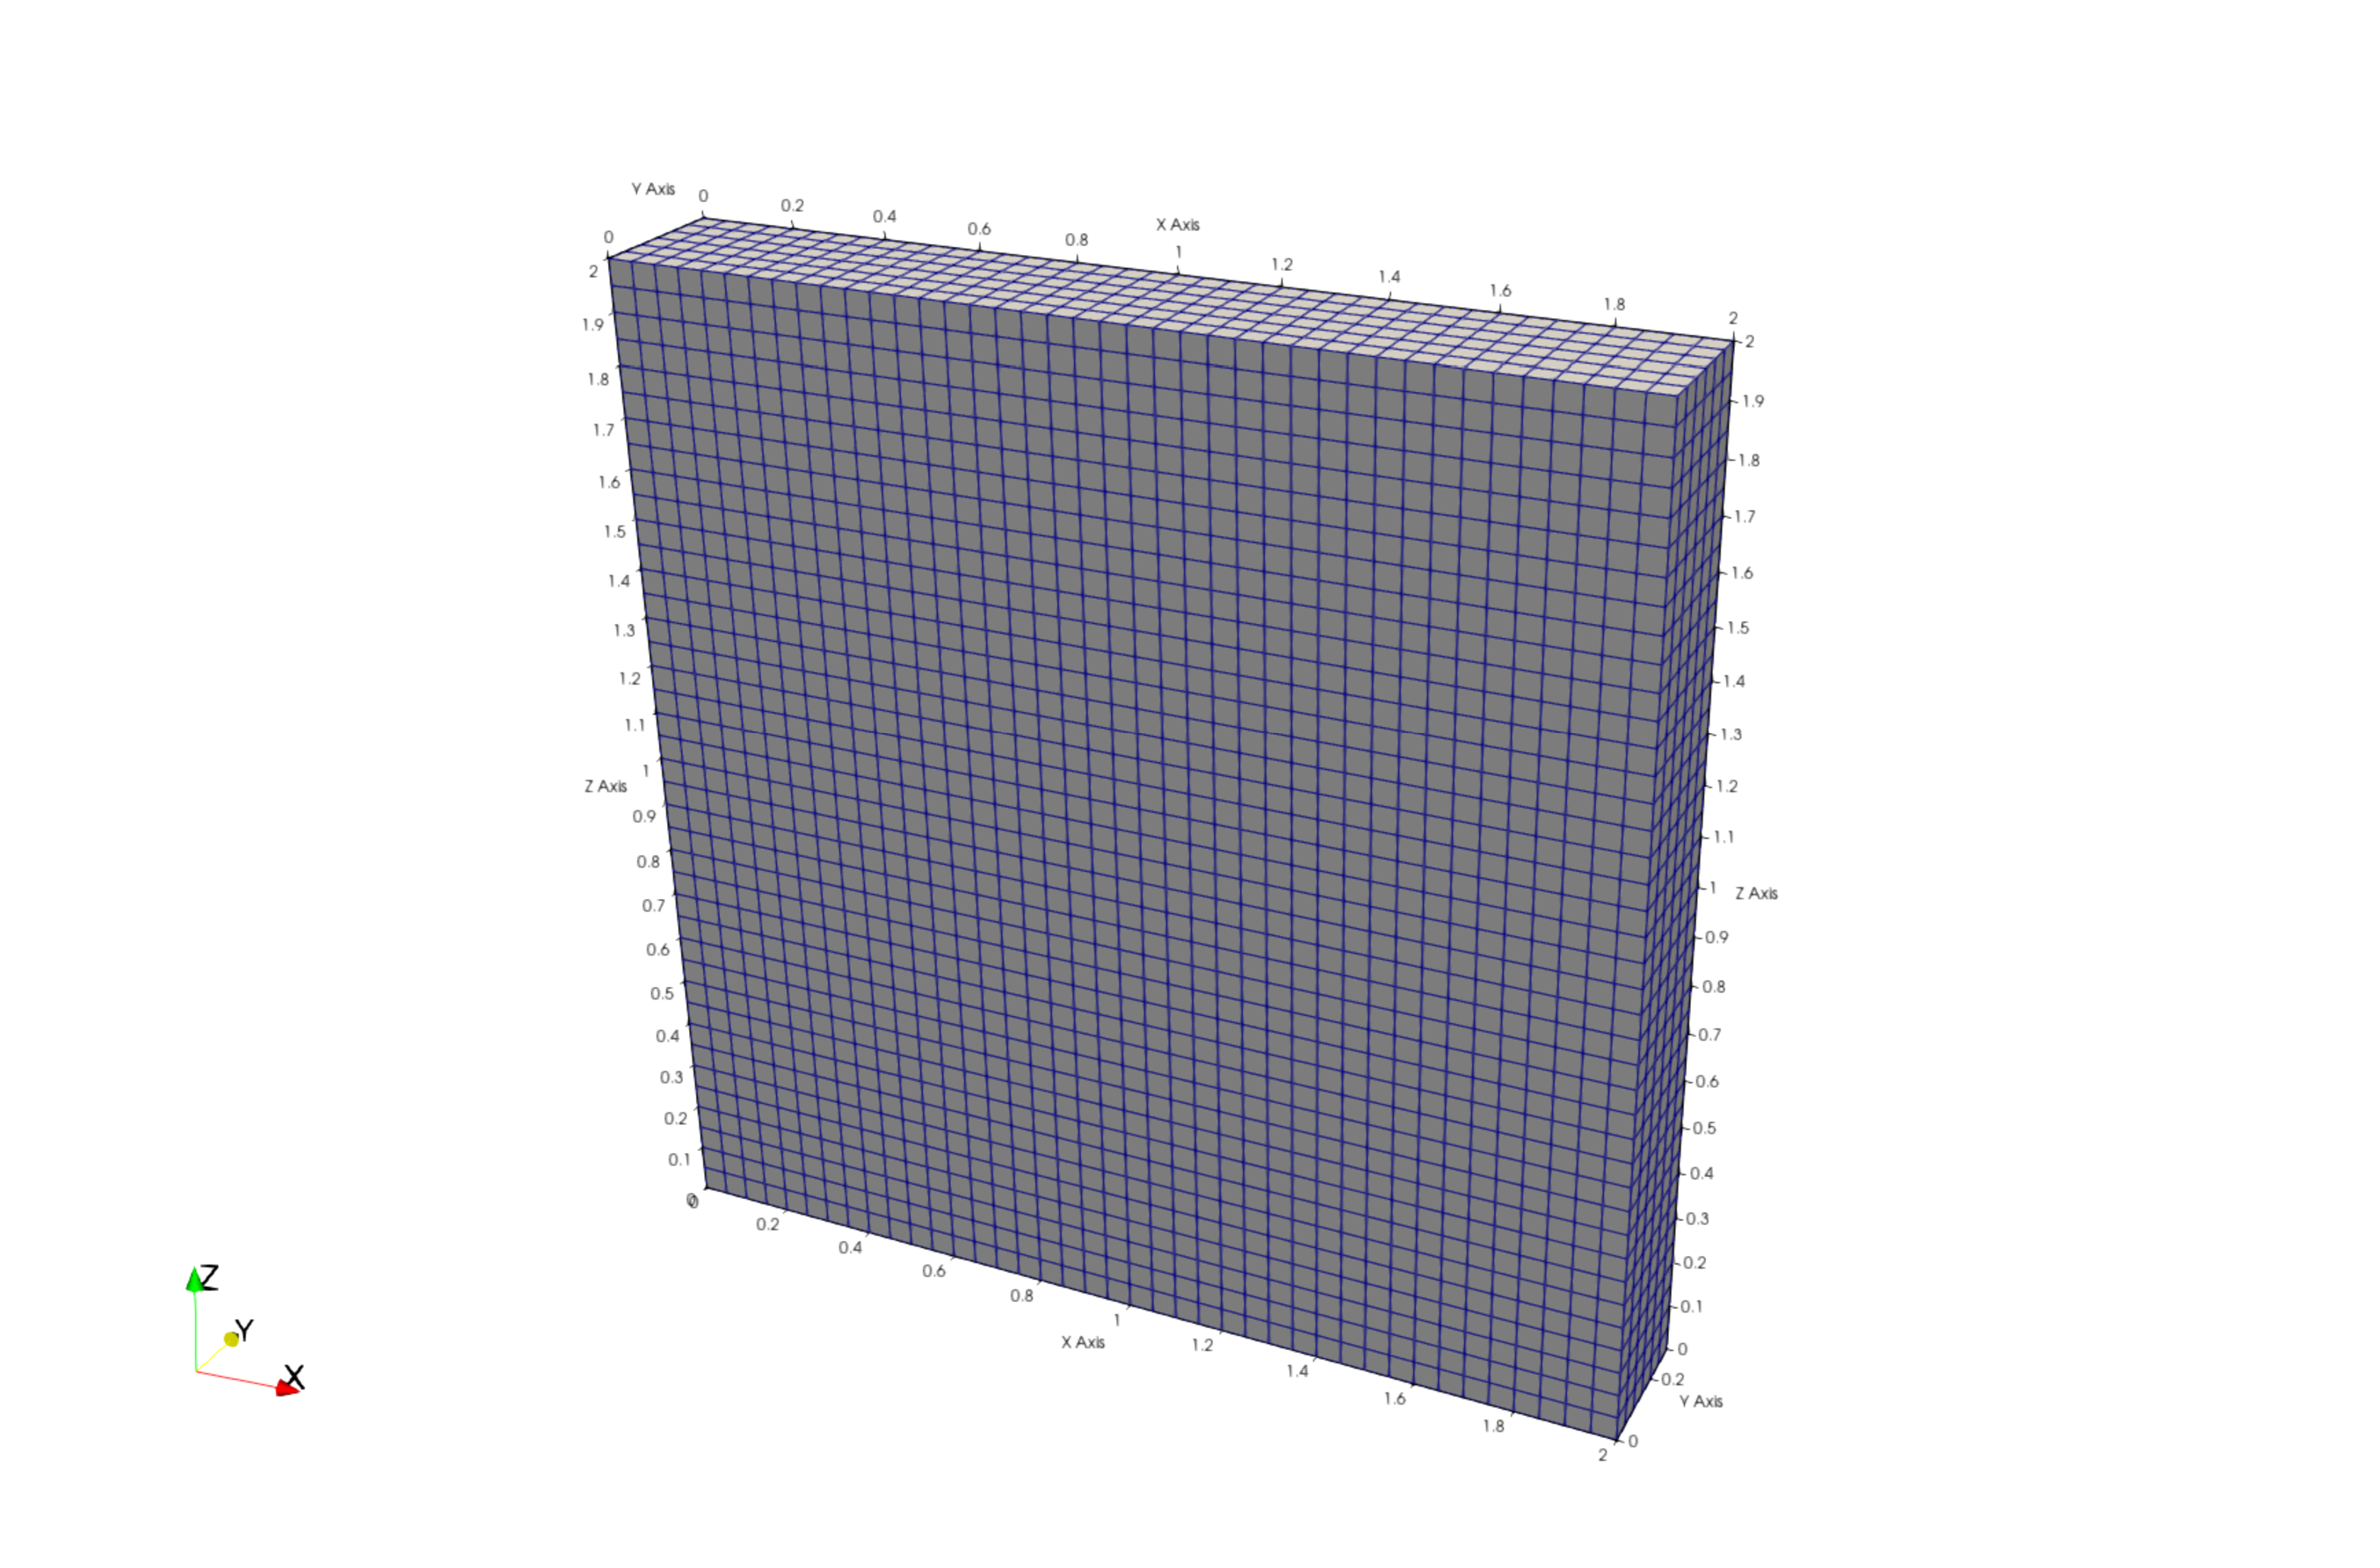
\includegraphics[width=10truecm]{pics/3d-dambreak/mesh.jpeg}
		\caption{ダムブレイクの計算メッシュ}
		\label{fig:3d-dambreak-mesh}
	\end{minipage}
	\begin{minipage}[b]{0.49\columnwidth}
	    \centering
		\includegraphics[width=10truecm]{pics/3d-dambreak/heaviside_init.jpeg}
		\caption{ダムブレイクの初期のレベルセット関数と境界条件。全面no-slip条件}
		\label{fig:3d-dambreak-boundary}
	\end{minipage}
\end{figure}

\newpage
\subsection{解析結果}

\begin{figure}[H]
	\centering
	\begin{minipage}[b]{0.19\columnwidth}
	    \centering
	    \includegraphics[width=3.5truecm]{pics/3d-dambreak/result_0000.jpeg}
	\end{minipage}
	\begin{minipage}[b]{0.19\columnwidth}
	    \centering
	    \includegraphics[width=3.5truecm]{pics/3d-dambreak/result_0010.jpeg}
	\end{minipage}
	\begin{minipage}[b]{0.19\columnwidth}
	    \centering
	    \includegraphics[width=3.5truecm]{pics/3d-dambreak/result_0020.jpeg}
	\end{minipage}
	\begin{minipage}[b]{0.19\columnwidth}
	    \centering
	    \includegraphics[width=3.5truecm]{pics/3d-dambreak/result_0030.jpeg}
	\end{minipage}
	\begin{minipage}[b]{0.19\columnwidth}
	    \centering
	    \includegraphics[width=3.5truecm]{pics/3d-dambreak/result_0040.jpeg}
	\end{minipage}

	\caption{ダムブレイクの結果}
	\label{fig:dambreak-result}
\end{figure}

\begin{figure}[H]
	\centering
	\begin{minipage}[b]{0.19\columnwidth}
	    \centering
	    \includegraphics[width=3.5truecm]{pics/3d-dambreak/result_0050.jpeg}
	\end{minipage}
	\begin{minipage}[b]{0.19\columnwidth}
	    \centering
	    \includegraphics[width=3.5truecm]{pics/3d-dambreak/result_0060.jpeg}
	\end{minipage}
	\begin{minipage}[b]{0.19\columnwidth}
	    \centering
	    \includegraphics[width=3.5truecm]{pics/3d-dambreak/result_0070.jpeg}
	\end{minipage}
	\begin{minipage}[b]{0.19\columnwidth}
	    \centering
	    \includegraphics[width=3.5truecm]{pics/3d-dambreak/result_0080.jpeg}
	\end{minipage}
	\begin{minipage}[b]{0.19\columnwidth}
	    \centering
	    \includegraphics[width=3.5truecm]{pics/3d-dambreak/result_0090.jpeg}
	\end{minipage}

	\caption{ダムブレイクの結果}
	\label{fig:dambreak-result}
\end{figure}

\begin{figure}[H]
	\centering
	\includegraphics[width=10truecm]{pics/3d-dambreak/dambreak_result_v_and_v.pdf}
	\caption{Referenceとの比較\cite{Martin1952}}
	\label{fig:3d-dambreak-result-comparison}
\end{figure}

\begin{figure}[H]
	\centering
	\includegraphics[width=4truecm]{pics/3d-dambreak/experiment_koshizuka1996.png}
	\caption{Referenceとの比較\cite{Koshizuka1996}}
	\label{fig:3d-dambreak-result-picture}
\end{figure}

\subsection{体積保存を入れない場合の結果}

\begin{figure}[H]
	\centering
	\begin{minipage}[b]{0.19\columnwidth}
	    \centering
	    \includegraphics[width=3.5truecm]{pics/3d-dambreak/no_volume_correction/result_0000.jpeg}
	\end{minipage}
	\begin{minipage}[b]{0.19\columnwidth}
	    \centering
	    \includegraphics[width=3.5truecm]{pics/3d-dambreak/no_volume_correction/result_0010.jpeg}
	\end{minipage}
	\begin{minipage}[b]{0.19\columnwidth}
	    \centering
	    \includegraphics[width=3.5truecm]{pics/3d-dambreak/no_volume_correction/result_0020.jpeg}
	\end{minipage}
	\begin{minipage}[b]{0.19\columnwidth}
	    \centering
	    \includegraphics[width=3.5truecm]{pics/3d-dambreak/no_volume_correction/result_0030.jpeg}
	\end{minipage}
	\begin{minipage}[b]{0.19\columnwidth}
	    \centering
	    \includegraphics[width=3.5truecm]{pics/3d-dambreak/no_volume_correction/result_0033.jpeg}
	\end{minipage}

	\caption{ダムブレイクの結果(体積保存を入れない場合)}
	\label{fig:dambreak-result}
\end{figure}


\subsection{レベルセット関数の最初期化を入れない場合の結果}

\begin{figure}[H]
	\centering
	\begin{minipage}[b]{0.19\columnwidth}
	    \centering
	    \includegraphics[width=3.5truecm]{pics/3d-dambreak/no_reinitialization/result_0000.jpeg}
	\end{minipage}
	\begin{minipage}[b]{0.19\columnwidth}
	    \centering
	    \includegraphics[width=3.5truecm]{pics/3d-dambreak/no_reinitialization/result_0010.jpeg}
	\end{minipage}
	\begin{minipage}[b]{0.19\columnwidth}
	    \centering
	    \includegraphics[width=3.5truecm]{pics/3d-dambreak/no_reinitialization/result_0020.jpeg}
	\end{minipage}
	\begin{minipage}[b]{0.19\columnwidth}
	    \centering
	    \includegraphics[width=3.5truecm]{pics/3d-dambreak/no_reinitialization/result_0030.jpeg}
	\end{minipage}
	\begin{minipage}[b]{0.19\columnwidth}
	    \centering
	    \includegraphics[width=3.5truecm]{pics/3d-dambreak/no_reinitialization/result_0040.jpeg}
	\end{minipage}

	\caption{ダムブレイクの結果(再初期化を入れない場合)}
	\label{fig:dambreak-result}
\end{figure}


\subsection{並列解析結果}
TBA。現状体積保存の所が並列化未対応。

\begin{comment}
本ソルバーは領域分割法によるMPI並列化にも対応しているため、
3.5項で示した並列化解析実行手順に従い並列数を4として並列解析をした結果を示す。

Figure \ref{fig:3d-dambreak-parallel-partition}に領域分割したメッシュを示す。

\begin{figure}[H]
	\centering
	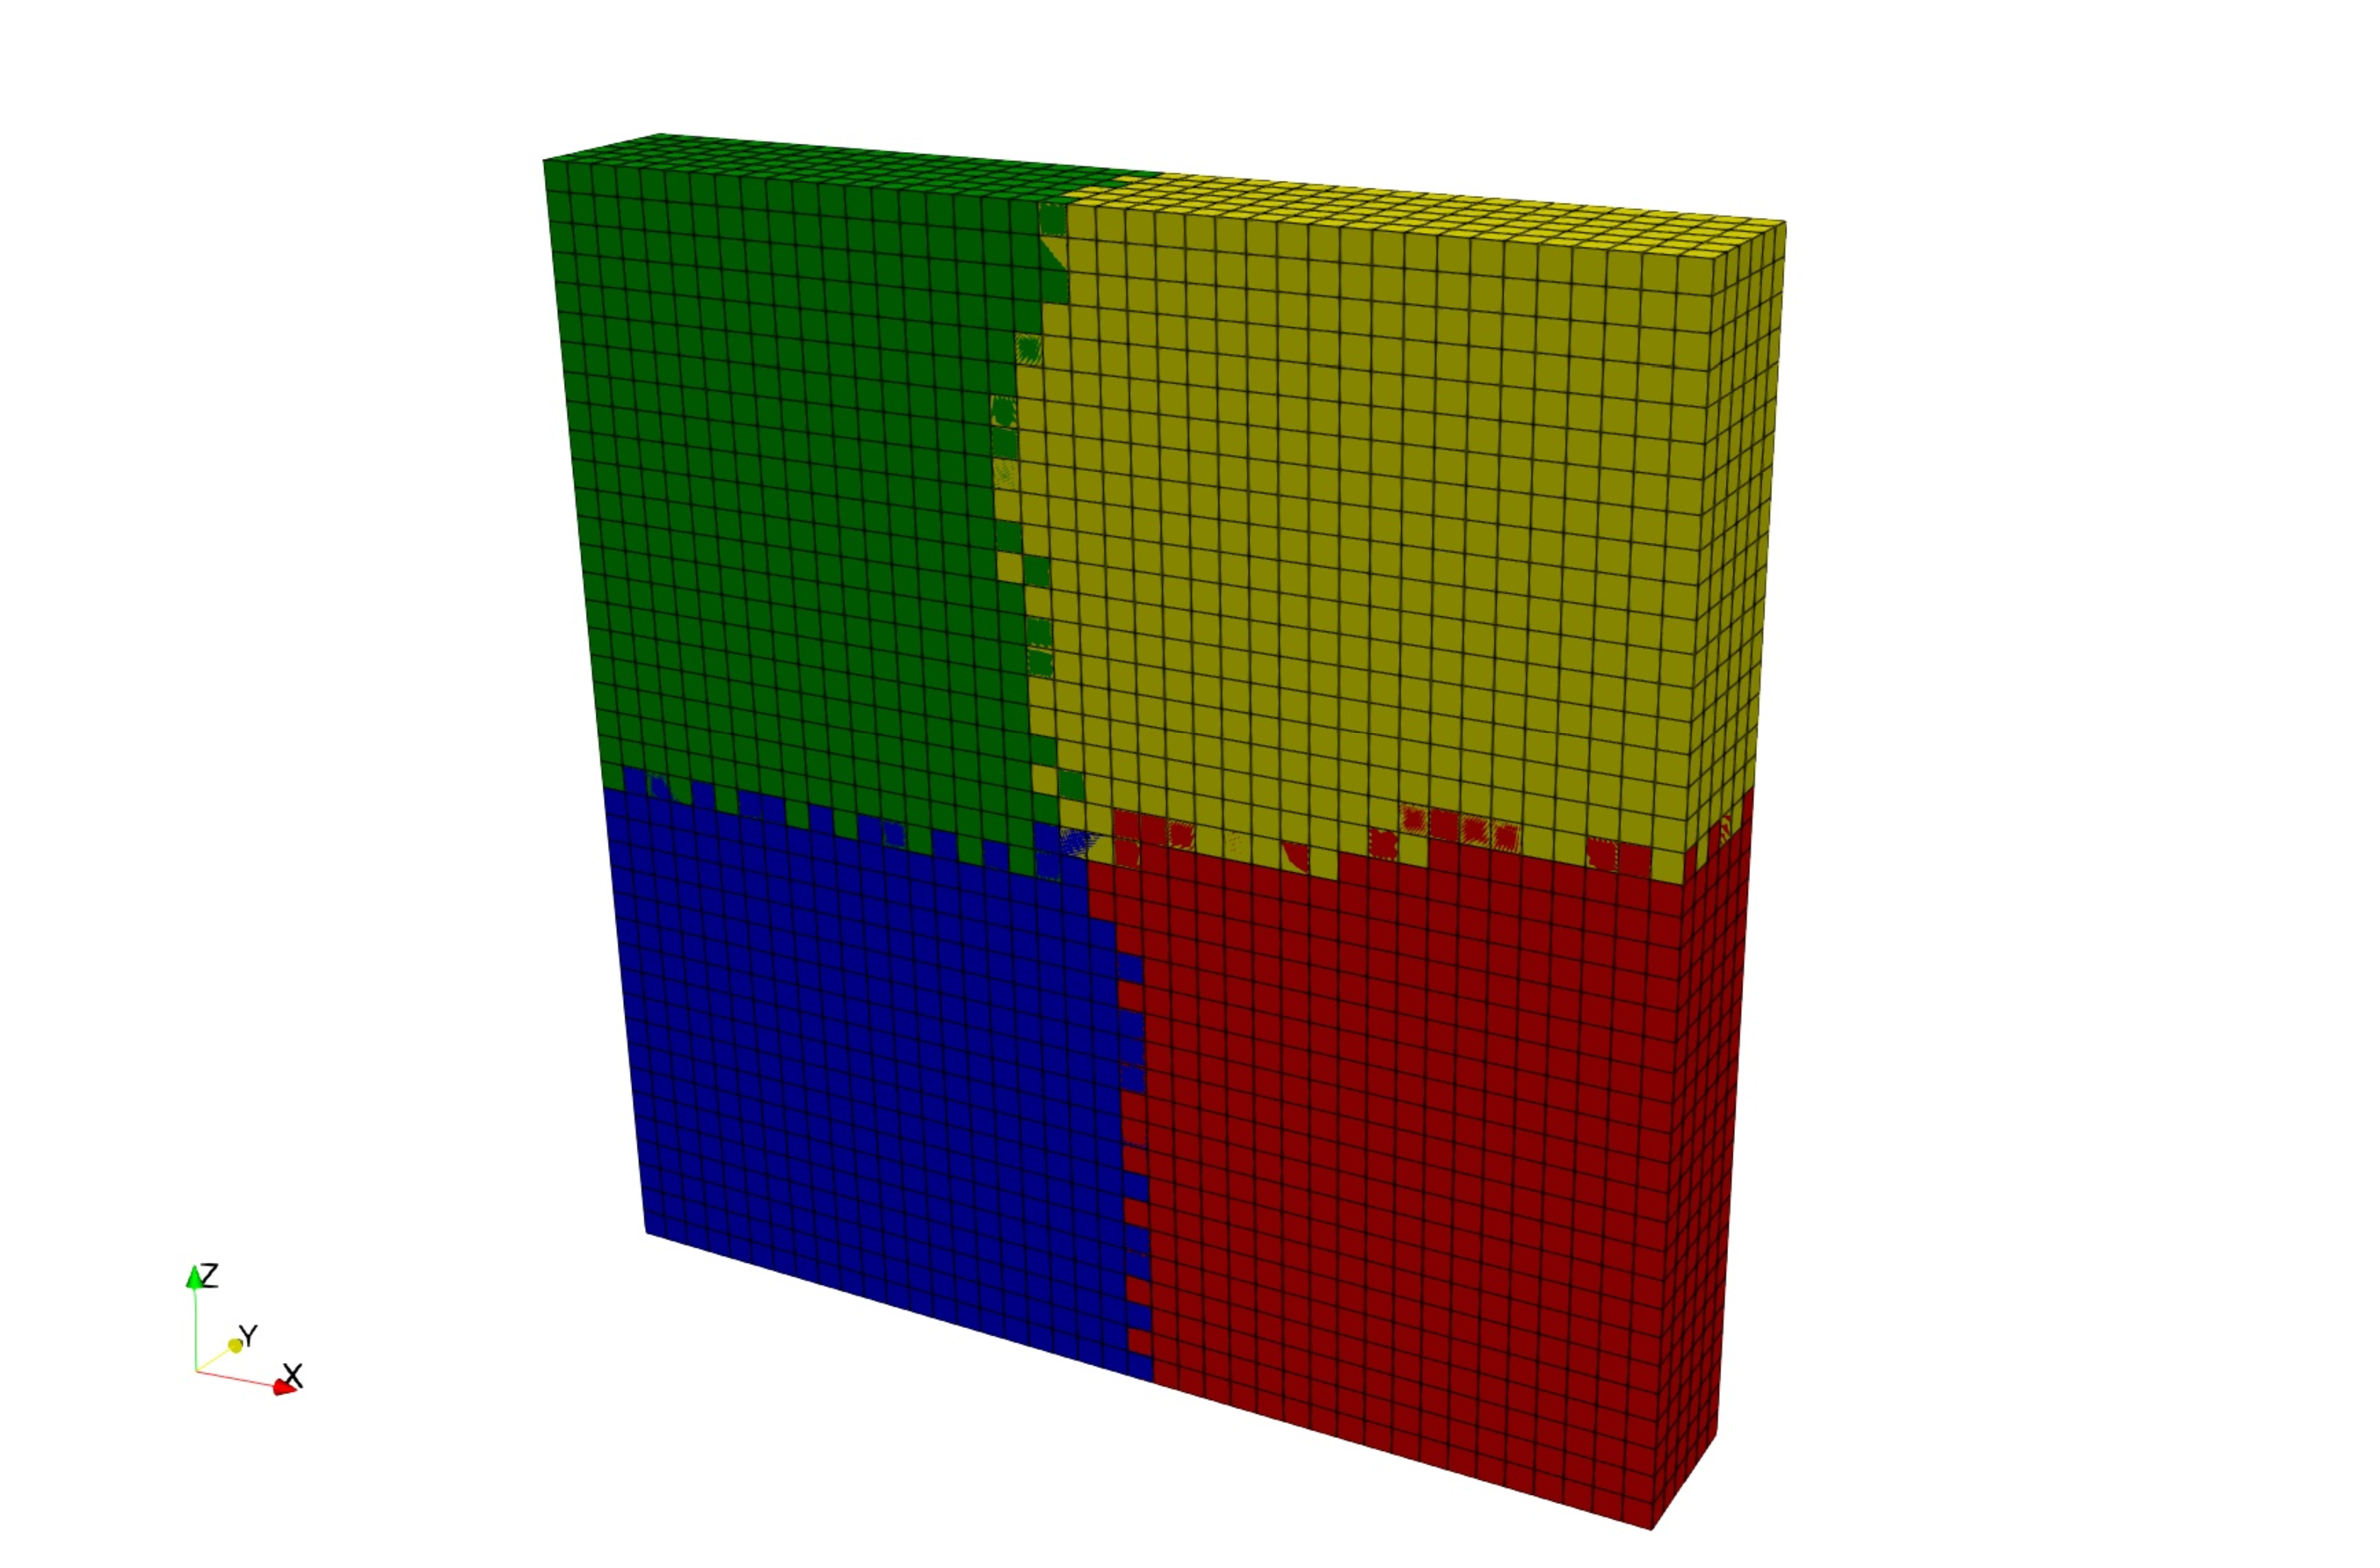
\includegraphics[width=10truecm]{pics/3d-dambreak-parallel/partition4.pdf}
	\caption{並列数4の場合の領域分割の図}
	\label{fig:3d-dambreak-parallel-partition}
\end{figure}


Figure \ref{fig:3d-dambreak-parallel-result}に速度分布、圧力分布、レベルセット関数の結果を示す。
並列化なしの場合と同様の結果が得られており、並列化解析が問題なくできていることが確認できた。
計算時間についても大幅に短くなっているが、時間計測は今回は行っていないため、今後スケーリング効果の計測を実施する。

\begin{figure}[H]
	\centering
	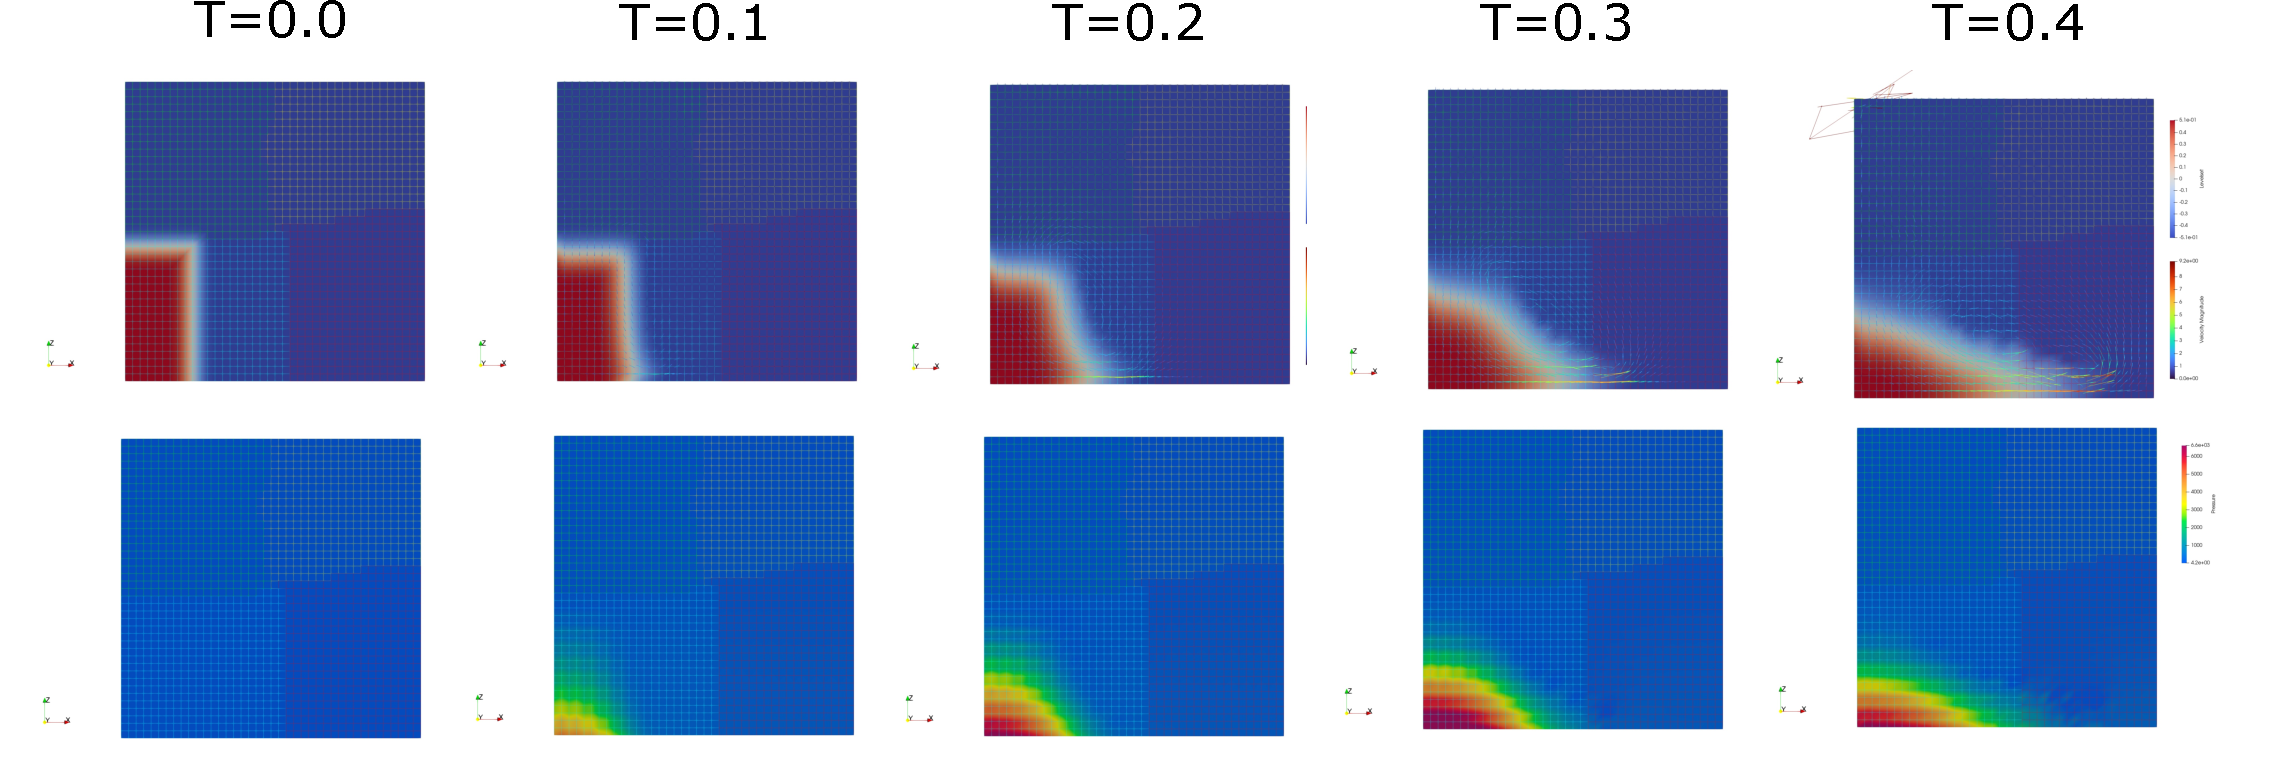
\includegraphics[width=18truecm]{pics/3d-dambreak-parallel/result-partition4.pdf}
	\caption{ダムブレイク問題のCase2の並列化解析による計算結果($y=0.4$における断面)。網目の色の違いで領域分割されている領域を可視化した。}
	\label{fig:3d-dambreak-parallel-result}
\end{figure}

ダムブレイクの検証\cite{Okumura2009}, 
有名な文献\cite{Koshizuka1996}
\end{comment}